\documentclass[aps,prb,twocolumn,floatfix,nofootinbib,superscriptaddress]{revtex4-2}

\usepackage{amsmath,amssymb,amsthm,mathtools,bm}
\usepackage{booktabs}
\usepackage{graphicx}
\usepackage[colorlinks=true,linkcolor=blue,citecolor=blue,urlcolor=blue]{hyperref}
\usepackage{microtype}

\newcommand{\Tr}{\operatorname{Tr}}
\newcommand{\tr}{\operatorname{tr}}
\newcommand{\E}{\mathbb{E}}

\begin{document}

\title{Many-body Lyapunov spectroscopy from maximally mixed Gaussian trajectories: Diagnostic results for the adaptive chiral wall}

\author{Asadullah Bhuiyan}
\date{September 4, 2026}

\begin{abstract}
We reconstruct the many-body singular spectrum of a resolved Gaussian trajectory from a maximally mixed input.  The normalized conditional output is the right Choi marginal, \(\hat V_{\boldsymbol m}\hat V_{\boldsymbol m}^{\dagger}/Z_{\boldsymbol m}\); its one-particle occupations generate the normalized many-body spectrum, while the accumulated Born probability restores \(Z_{\boldsymbol m}\).  We apply this construction to 800 independent Born trajectories at \(N_x=20\), eight circumferences \(N_y=20\)--40, and depth \(T=2N_y\).  All 160 task products pass checksum, provenance, reconstruction, cycle-completeness, exact-cap, and numerical-residual checks.  Late-window record-weight slopes agree with the leading spectral slopes to better than 0.3\% at every size, and the first four soft modes carry 95--97\% of their transverse weight near the two walls.  However, every circumference fails at least one preregistered middle-to-late stability test.  The leading \(1/N_y^2\) coefficient has the wrong sign, a confidence interval containing zero, and extreme fit-window sensitivity.  The campaign therefore validates the Gaussian spectrum reconstruction and its boundary localization, but it does not support a precision effective-central-charge or absolute operator-dimension extraction.  We recommend, but do not launch, a fresh \(T=4N_y\) depth study at \(N_y=20,30,40\).
\end{abstract}

\maketitle
\setcounter{tocdepth}{2}
\tableofcontents

\section{Question and short answer}

For a fixed measurement record \(\boldsymbol m\), the monitored circuit defines one resolved many-body evolution operator (mEO) \(\hat V_{\boldsymbol m}(t)\).  Zabalo \emph{et al.} call the corresponding trajectory operator \(K_{\boldsymbol m}\); we retain \(\hat V_{\boldsymbol m}\) for the project's canonical mEO notation and use their notation for its singular values and Lyapunov exponents.  We want the leading many-body singular values and their long-time Lyapunov rates without constructing an exponentially large Fock-space matrix.

The term here is \emph{many-body Lyapunov spectrum}.  It is not a Lieb--Robinson velocity or spectrum: Lieb--Robinson bounds constrain how rapidly information can propagate in space, whereas Lyapunov exponents describe the exponential growth or decay of singular values of a long operator product.

The answer is particularly simple for a Gaussian circuit.  Evolve the maximally mixed state along the resolved record, diagonalize the resulting one-particle covariance, and retain the cumulative Born log probability of that same record.  The covariance occupations determine every \emph{relative} many-body singular value; the scalar Born weight supplies their common absolute normalization.  Thus one Gaussian trajectory contains the complete many-body singular spectrum of the corresponding resolved mEO.

Throughout this note we follow the notation of Zabalo \emph{et al.}: \(\sigma_i^{\boldsymbol m}(t)\) is a finite-time singular value and \(\lambda_i^{\boldsymbol m}\) is its squared-singular-value growth rate,
\begin{equation}
 [\sigma_i^{\boldsymbol m}(t)]^2
 =\exp\!\left[t\lambda_i^{\boldsymbol m}+o(t)\right].
 \label{eq:zabalo-convention}
\end{equation}
This convention prevents an otherwise common factor-of-two ambiguity.  In informal discussion the word ``spectrum'' may refer to either \(\sigma_i\) or \(\lambda_i\); below the notation always distinguishes them.

\section{Resolved trajectory and maximally mixed probe}

Let \(N=2N_xN_y\) be the number of complex fermion modes, including the two orbitals per unit cell.  A resolved record through circuit depth \(t\) is \(\boldsymbol m=(m_1,\ldots,m_t)\), including every measurement outcome needed to determine the feedback operations.  Its chronological operator is
\begin{equation}
 \hat V_{\boldsymbol m}(t)
 =\hat K_{m_t}\cdots \hat K_{m_2}\hat K_{m_1}.
 \label{eq:record-operator}
\end{equation}
No sum over records is taken.  Any nonnegative positive-operator-valued-measure (POVM) weight is understood to be absorbed into the corresponding resolved Kraus operator \(\hat K_m\).

Use the full-Fock-space maximally mixed input
\begin{equation}
 \hat\rho_*=\frac{\hat{\mathbf{1}}}{2^N}.
 \label{eq:maxmix}
\end{equation}
The probability of obtaining \(\boldsymbol m\) from this input is
\begin{equation}
 p_{\boldsymbol m}(t)
 =\Tr\!\left[
 \hat V_{\boldsymbol m}(t)\hat\rho_*\hat V_{\boldsymbol m}^{\dagger}(t)
 \right]
 =\frac{Z_{\boldsymbol m}(t)}{2^N},
 \label{eq:born-z}
\end{equation}
where
\begin{equation}
 Z_{\boldsymbol m}(t)
 =\Tr\!\left[
 \hat V_{\boldsymbol m}(t)\hat V_{\boldsymbol m}^{\dagger}(t)
 \right].
 \label{eq:zk}
\end{equation}
The normalized conditional output is therefore
\begin{equation}
 \hat\rho^V_{R,\boldsymbol m}(t)
 =\frac{
 \hat V_{\boldsymbol m}(t)\hat V_{\boldsymbol m}^{\dagger}(t)
 }{Z_{\boldsymbol m}(t)}.
 \label{eq:right-choi}
\end{equation}
This is the right marginal of the normalized trajectory Choi state.  The maximally mixed input is consequently a spectroscopic device, not a claim about the physical state prepared in the experiment.

Equation~\eqref{eq:born-z} also gives the scalar information that normalized covariance dynamics discards.  If the simulator accumulates
\begin{equation}
 \omega_{\boldsymbol m}(t)=\log p_{\boldsymbol m}(t)
 =\sum_{u\leq t}\log p(m_u\mid m_1,\ldots,m_{u-1}),
 \label{eq:logweight}
\end{equation}
then
\begin{equation}
 \boxed{\log Z_{\boldsymbol m}(t)=N\log 2+\omega_{\boldsymbol m}(t).}
 \label{eq:logz}
\end{equation}
The same realized record must supply both the covariance and \(\omega_{\boldsymbol m}\).

\section{Exact Gaussian reconstruction}

For the number-conserving right state in Eq.~\eqref{eq:right-choi}, define the normal covariance
\begin{equation}
 G_{ij}^{\boldsymbol m}(t)
 =\Tr\!\left[
 \hat\rho^V_{R,\boldsymbol m}(t)\hat c_i^{\dagger}\hat c_j
 \right].
 \label{eq:normal-covariance}
\end{equation}
Let \(\nu_a^{\boldsymbol m}(t)\in[0,1]\), \(a=1,\ldots,N\), be its occupation eigenvalues.  In the corresponding natural-orbital basis the Gaussian state factorizes, so a binary occupation string \(\bm n=(n_1,\ldots,n_N)\), with each \(n_a=0\) or \(1\), has normalized many-body weight
\begin{equation}
 w_{\bm n}^{\boldsymbol m}(t)
 =\prod_{a=1}^{N}
 [\nu_a^{\boldsymbol m}(t)]^{n_a}
 [1-\nu_a^{\boldsymbol m}(t)]^{1-n_a}.
 \label{eq:fock-products}
\end{equation}
Since these are the eigenvalues of Eq.~\eqref{eq:right-choi}, the squared singular values and singular values of the resolved mEO are
\begin{align}
 [\sigma_{\bm n}^{\boldsymbol m}(t)]^2
 &=Z_{\boldsymbol m}(t)w_{\bm n}^{\boldsymbol m}(t),
 \label{eq:squared-singular-values}\\
 \sigma_{\bm n}^{\boldsymbol m}(t)
 &=\sqrt{Z_{\boldsymbol m}(t)}
 \prod_{a=1}^{N}
 [\nu_a^{\boldsymbol m}(t)]^{n_a/2}
 [1-\nu_a^{\boldsymbol m}(t)]^{(1-n_a)/2}.
 \label{eq:singular-values}
\end{align}
Equations~\eqref{eq:logz} and \eqref{eq:singular-values} define the extraction used below.  They remain valid for a nonzero exact projective branch of definite U(1) charge because \(\hat V_{\boldsymbol m}\hat V_{\boldsymbol m}^{\dagger}\) is neutral, even when \(\hat V_{\boldsymbol m}\) itself changes charge.

\subsection{What the calculation actually does}

For each independent sample, the numerical operation is:
\begin{enumerate}
 \item initialize the one-particle correlation matrix as \(G(0)=\tfrac12\mathbf{1}_N\);
 \item generate one complete record with the Born rule while applying its adaptive feedback, and accumulate the realized \(\omega_{\boldsymbol m}(t)\) in Eq.~\eqref{eq:logweight};
 \item at the chosen cycle checkpoints, diagonalize \(G^{\boldsymbol m}(t)\) to obtain \(\nu_a^{\boldsymbol m}(t)\) and the natural orbitals;
 \item recover \(\log Z_{\boldsymbol m}(t)\) from Eq.~\eqref{eq:logz};
 \item construct the leading ordered \(\ell_i^{\boldsymbol m}(t)=\log[\sigma_i^{\boldsymbol m}(t)]^2\) using Eq.~\eqref{eq:leading-level} and the smallest flip-cost sums; and
 \item fit the checkpoint dependence to obtain one set of trajectory Lyapunov rates, then average those rates over independent records and fit their \(N_y\) dependence.
\end{enumerate}
No exponentially large many-body matrix is stored.  A record generated from a different initial state may still be replayed to reconstruct the spectrum of that particular \(\hat V_{\boldsymbol m}\), but such records are sampled from the wrong measure for the simple Born average in Eq.~\eqref{eq:born-average}.  The completed ensemble therefore generated the records from the maximally mixed input itself.

\subsection{Ordering the leading levels without exponential work}

We never enumerate all \(2^N\) binary strings.  For every natural mode define its preferred and suppressed weights
\begin{equation}
 q_a=\max(\nu_a,1-\nu_a),
 \qquad
 r_a=\min(\nu_a,1-\nu_a),
 \label{eq:preferred}
\end{equation}
and its positive flip cost
\begin{equation}
 d_a=\log\frac{q_a}{r_a}
 =\left|\log\frac{\nu_a}{1-\nu_a}\right|.
 \label{eq:flip-cost}
\end{equation}
The largest many-body weight selects the preferred choice in every mode:
\begin{equation}
 \log[\sigma_0^{\boldsymbol m}(t)]^2
 =\log Z_{\boldsymbol m}(t)+\sum_a\log q_a.
 \label{eq:leading-level}
\end{equation}
The next levels are obtained by flipping one or more natural-mode choices.  Every flip subtracts its \(d_a\) from Eq.~\eqref{eq:leading-level}.  Sorting the smallest sums of the \(d_a\)'s therefore produces the leading \(M\) many-body levels with a standard heap algorithm whose cost is polynomial in \(N\) and \(M\).  In the production analysis we initially need only \(M\sim16\)--\(64\), not the complete exponentially long list.

If \(\nu_a=0\) or \(1\) exactly, that mode is a sharp empty or occupied Choi cap.  Its preferred factor is one and its suppressed factor is zero.  Flipping it produces a genuine zero singular value and a Lyapunov exponent \(-\infty\).  Exact caps must not be turned into finite gaps by numerical clipping.  If a fixed-particle-number block of the mEO is desired instead of the full Fock-space spectrum, Eq.~\eqref{eq:fock-products} is restricted to binary strings with the required particle number; the lowest changes are then particle--hole replacements.

\subsection{Related tangent quantities are not substitutes}

The identity-input covariance half-Jacobian has one-leg singular values
\begin{equation}
 j_a=2\sqrt{\nu_a(1-\nu_a)}.
 \label{eq:half-jacobian}
\end{equation}
These bounded numbers contain the same unoriented radial information, but the full covariance Jacobian has pairwise singular values \(j_aj_b\); those are not the many-body singular values in Eq.~\eqref{eq:singular-values}.  Likewise, a tangent calculation about a pure Slater trajectory sees only the coherent one-particle--one-hole sector.  The maximally mixed construction is the appropriate object when the target is the complete normalized many-body spectrum of the resolved operator.

\section{Lyapunov exponents and record free energy}

At several depths, compute the ordered logarithms
\begin{equation}
 \ell_i^{\boldsymbol m}(t)=\log[\sigma_i^{\boldsymbol m}(t)]^2.
 \label{eq:ell}
\end{equation}
For each independent trajectory, fit
\begin{equation}
 \ell_i^{\boldsymbol m}(t)=b_i^{\boldsymbol m}+t\lambda_i^{\boldsymbol m}
 \label{eq:trajectory-fit}
\end{equation}
inside a stationary window.  The intercept absorbs the fixed \(N\log2\) term and finite-depth preparation effects.  The Born-ensemble exponent is
\begin{equation}
 \lambda_i(L)=\E_{\boldsymbol m}\!\left[\lambda_i^{\boldsymbol m}(L)\right].
 \label{eq:born-average}
\end{equation}
Records generated with the simulator's Born rule are already sampled from the required distribution.  Their trajectory estimates receive an ordinary arithmetic mean; they are not multiplied by a second Born weight.

The Shannon entropy of the measurement record is
\begin{equation}
 F(L,t)
 =-\sum_{\boldsymbol m}p_{\boldsymbol m}(t)\log p_{\boldsymbol m}(t)
 =\E_{\boldsymbol m}[-\omega_{\boldsymbol m}(t)].
 \label{eq:free-energy}
\end{equation}
At long depth, Zabalo \emph{et al.} identify
\begin{equation}
 \frac{F(L,t)}{t}\longrightarrow-\lambda_0(L).
 \label{eq:f-lambda0}
\end{equation}
At finite depth our Gaussian reconstruction supplies the more exact leading quantity through Eq.~\eqref{eq:leading-level}.  Saving the realized \(\omega_{\boldsymbol m}\), rather than only the sum of binary entropies of possible outcomes, also permits recordwise covariance between free energy and spectral gaps.

The positive finite-time gap from the leading level is especially transparent:
\begin{multline}
 \ell_0^{\boldsymbol m}(t)-\ell_i^{\boldsymbol m}(t)\\
 =\text{the corresponding ordered sum of }d_a(t).
 \label{eq:ordered-gap}
\end{multline}
The normalization \(Z_{\boldsymbol m}\) cancels from this difference, but it remains indispensable for \(\lambda_0\), \(F\), and the effective-central-charge analysis.

\section{Following Zabalo Eqs.~(3) and (4)}

For a one-dimensional critical transfer problem on a cylinder of circumference \(L\), Zabalo \emph{et al.} define
\begin{equation}
 f_i(L)=-\frac{\lambda_i(L)}{\alpha L}.
 \label{eq:fi}
\end{equation}
Their leading finite-size forms are
\begin{align}
 f_0(L)&=f_\infty-\frac{\pi c_{\mathrm{eff}}}{6L^2}+\cdots,
 \label{eq:zabalo3}\\
 f_i(L)-f_0(L)&=\frac{2\pi x_i^{\mathrm{typ}}}{L^2}+\cdots.
 \label{eq:zabalo4}
\end{align}
The completed analysis directly tests Eqs.~\eqref{eq:zabalo3} and \eqref{eq:zabalo4}.  Ratios of gaps are not a replacement for this analysis and are not part of the primary extraction.  They are retained only when their underlying finite-size coefficients pass independently.

\subsection{What is and is not required about \texorpdfstring{\(\alpha\)}{alpha}}

No anisotropy is needed to run the circuit, reconstruct \(\sigma_i\), fit \(\lambda_i\), or estimate the record free energy.  It enters only when a decay rate measured per circuit cycle is converted into the conventional absolute CFT normalization in Eqs.~\eqref{eq:zabalo3} and \eqref{eq:zabalo4}.  Thus \(\alpha\) need not be known \emph{a priori}; all raw spectral data can be collected first.

There is nevertheless no mathematical justification for silently deleting \(\alpha\) while claiming an independent absolute \(c_{\mathrm{eff}}\) or \(x_i\).  If we work directly in the fixed cycle convention, define
\begin{equation}
 \widetilde f_i(L)=-\frac{\lambda_i(L)}{L}=\alpha f_i(L).
 \label{eq:raw-fi}
\end{equation}
Then the leading \(1/L^2\) coefficient measures \(\alpha c_{\mathrm{eff}}\), and the excited coefficients measure \(\alpha x_i^{\mathrm{typ}}\).

There is also an exact way to remove \(\alpha\) without abandoning Zabalo's finite-size relations.  Let \(A_0\) be the fitted coefficient of \(1/L^2\) in \(\widetilde f_0\), and let \(A_i\) be that coefficient in \(\widetilde f_i-\widetilde f_0\).  Equations~\eqref{eq:zabalo3} and \eqref{eq:zabalo4} imply
\begin{equation}
 \frac{x_i^{\mathrm{typ}}}{c_{\mathrm{eff}}}
 =-\frac{A_i}{12A_0}.
 \label{eq:slope-ratio}
\end{equation}
This is a ratio of independently extrapolated finite-size coefficients, not a ratio of raw level gaps at one size.

For the present project this is enough.  The spatial entanglement calculation already estimates the wall central charge without any time-to-space conversion.  The legacy atlas finds a two-wall coefficient close to \(c=1\), together with the expected algebraic wall correlator.  Combining that spatial value with Eq.~\eqref{eq:slope-ratio} gives \(x_i^{\mathrm{typ}}\) without ever specifying \(\alpha\).  The Lyapunov free-energy fit then tests the expected finite-size form but does not provide an independent absolute value of \(c_{\mathrm{eff}}\).  If such an independent Lyapunov-only value is required, a separate correlation or aspect-ratio determination of \(\alpha\) must be added later.

\section{What boundary criticality changes}

The stochastic circuit is two-dimensional, but its soft critical sector is confined to interfaces running along the periodic \(y\) direction.  The effective conformal cylinder therefore uses
\begin{align}
 L&=N_y,\\
 N_x&=\text{fixed},\qquad N_x\gg\xi_{\mathrm{wall}}.
 \label{eq:boundary-geometry}
\end{align}
Gapped bulk degrees of freedom contribute to the nonuniversal term \(f_\infty\).  At fixed \(N_x\), their finite-\(N_y\) corrections should be exponential rather than the wall's universal \(1/N_y^2\) term.  A matched uniform control is useful for diagnosing or subtracting residual bulk contributions, but it does not alter the reconstruction formulas.

The periodic domain-wall geometry contains two interfaces with opposite chirality.  The atlas's full-strip entropy convention counts their combined critical content, while a contour isolating one interface carries half the logarithmic coefficient.  The mEO fit must use the same convention.  If the full operator contains two decoupled wall sectors, the low spectrum should show the corresponding paired structure and Eq.~\eqref{eq:zabalo3} returns the combined two-wall \(c_{\mathrm{eff}}\).  Any division into a per-wall value requires an explicit localization and wall-decoupling check.

The full spectrum also contains many exactly capped directions and strongly gapped bulk modes.  To identify the CFT levels rather than merely list ordered numbers, the natural orbitals associated with the smallest finite flip costs should be classified by
\begin{enumerate}
 \item transverse weight near each wall;
 \item momentum along \(y\), when translation resolution is available;
 \item U(1) charge sector and particle--hole content; and
 \item symmetric or antisymmetric combinations of the two walls.
\end{enumerate}
The occupation eigenvalues alone determine the ordered spectrum, but their eigenvectors or symmetry-resolved blocks are needed to name the corresponding operators and organize conformal towers.

\section{Completed v2 campaign and analysis}

The completed campaign uses
\begin{align}
 N_x&=20,\\
 N_y&=20,22,24,26,28,30,36,40,\\
 T&=2N_y,\qquad S=100\ \text{per }N_y.
 \label{eq:pilot-grid}
\end{align}
Every trajectory has the hard support-truncated domain wall at \(x=5,15\), \(n_{\rm shell}=1\), \(\alpha_1=1\), \(\alpha_2=30\), maximally mixed initialization, raster-\(y\) active-slab measurements, and perfect correction without postselection.  The executed A100 code used the canonical complex128 GPU entry point \texttt{classA\_U1FGTN\_gpu.run\_markov\_circuit}.  The 800 independent Born records are grouped into 160 tasks of five trajectories.

The observer saved \(\omega_{\boldsymbol m}(t)\) at every cycle and diagonalized the active correlation matrix at
\begin{equation}
 \{0,4,8,\ldots,2N_y\}\cup\{N_y,3N_y/2,2N_y\}.
 \label{eq:pilot-checkpoints}
\end{equation}
The active transfer space contains \(N_{\rm eff}=22N_y\) modes.  The saved convention is
\begin{align}
 \ell_i(t)&=\log [\sigma_i(t)]^2,\\
 d_a(t)&=\left|\log\frac{\nu_a(t)}{1-\nu_a(t)}\right|,\\
 \log Z_{\boldsymbol m}(t)&=N_{\rm eff}\log 2+\omega_{\boldsymbol m}(t).
 \label{eq:pilot-squared-convention}
\end{align}
Exact \(\nu_a=0,1\) caps retain infinite flip cost.  We reconstructed all 64 saved leading levels from the occupations and \(\log Z\); exact-cap-induced \(-\infty\) padding is excluded from time fits rather than converted into finite levels.

\subsection{Historical provenance and numerical validation}

The local data import contains 160 NPZ files and 160 completion JSON files.  We rehashed all 320 files, checked every task/configuration identity and all 800 global sample indices, and reproduced the download-manifest inventory digest.  Historical products are verified against the executed source hashes pinned in the import manifest.  A later repository update changed the current GPU engine hash, which is recorded separately and does not invalidate the immutable v2 products.  The largest observed Hermiticity, eigensolver, eigenvector-Gram, occupation-bound, active--exterior coupling, and exterior-product residuals are respectively $0$, $3.82\times10^{-15}$, $1.47\times10^{-14}$, $2.40\times10^{-11}$, $0$, and $0$.  All lie below their locked tolerances.

\subsection{Time-window and record-weight tests}

Each trajectory is fit separately in the middle and late windows \([N_y,3N_y/2]\) and \([3N_y/2,2N_y]\); only then are the slopes averaged.  Uncertainties are paired, stratified, whole-trajectory bootstrap intervals with 2000 replicates.  The criterion requires the shift interval to contain zero and the magnitude to be below 10\% for \(\lambda_0\) and the first four gaps.  Every circumference fails at least one of these five tests.  For example, the failed metric sets are \(\{\lambda_0,\Delta_3\}\) at \(N_y=20\), \(\{\lambda_0,\Delta_3\}\) at \(N_y=30\), and \(\{\Delta_1,\Delta_2,\Delta_3\}\) at \(N_y=40\).  Thus \(T=2N_y\) is not accepted as a stationary Lyapunov window.

The record check must compare like with like.  We therefore compare the late-window slope $d\omega/dt$ with \(\lambda_0\), rather than comparing the endpoint ratio \(-\omega(2N_y)/(2N_y)\) with a window slope.  The relative discrepancy is below $0.30\%$ at every size (and below $0.15\%$ at seven of eight sizes).  This is strong closure of the reconstructed normalization.  The endpoint ratio is retained only as a finite-depth diagnostic because its extensive intercept has not decayed by $2N_y$.

\subsection{Boundary localization}

Individual natural eigenvectors may rotate within nearly degenerate subspaces, so we do not attach stable wall labels to them.  Instead we average the projector weight of the first four soft modes in fixed two-column windows around both walls.  The combined fraction ranges from $0.9583$ to $0.9688$; all eight 95\% bootstrap lower bounds exceed $0.947$.  This validates a boundary-localized soft subspace without assigning momentum, charge, parity, or conformal-operator names.

\begin{figure*}[t]
 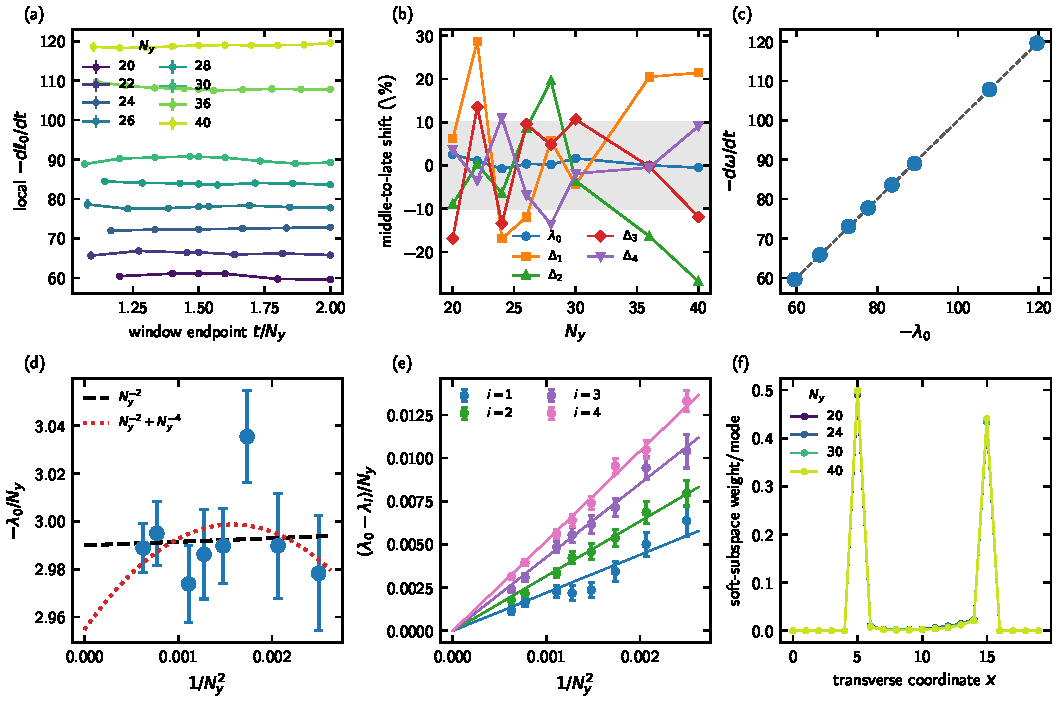
\includegraphics[width=\textwidth]{../../final_production_new_designs/04_maxmix_manybody_lyapunov_pilot/analysis_outputs/maxmix_manybody_lyapunov_nx20_ny20to40_s100_gpu_v2/many_body_lyapunov_v2_diagnostic.pdf}
 \caption{Completed v2 many-body Lyapunov diagnostic.  The ensemble contains $S=100$ independent Born trajectories at each $N_y$, maximally mixed initialization, and total depth $T=2N_y$.  Slopes are fit trajectory by trajectory before averaging.  (a) Local leading-level slopes; error bars are trajectory standard errors.  (b) Middle-to-late relative shifts for \(\lambda_0\) and four ordered gaps; the gray band is the 10\% magnitude condition, which is necessary but not sufficient because the paired 95\% bootstrap interval must also contain zero.  (c) Same-late-window record-weight and leading-level slopes.  (d) \(-\lambda_0/N_y\) with the all-size $N_y^{-2}$ fit and $N_y^{-4}$ sensitivity.  (e) Ordered gap densities with zero-intercept $N_y^{-2}$ fits.  (f) Aggregate first-four-mode transverse profiles; peaks occur at the two walls.  Finite-size fits use $N_y=20,22,24,26,28,30,36,40$; bootstrap uncertainties use 2000 whole-trajectory replicates.}
 \label{fig:v2-diagnostic}
\end{figure*}

\section{Finite-size diagnostic and claim gates}

The all-size fit of Eq.~\eqref{eq:raw-fi} gives
\begin{equation}
 A_0=+1.507,qquad A_0^{95\%}=[-19.97,24.87].
\end{equation}
The sign is opposite to that required for positive \(\alpha c_{\rm eff}\), the interval contains zero, and the regression has $R^2=0.0026$.  More importantly, the coefficient is not stable: adding $1/N_y^4$ changes it to $55.50$, while successive $N_{y,\min}$ fits change both its magnitude and sign.  The maximum sensitivity is about $35.8$ times the all-size coefficient, far above the preregistered 20\% bound.  The formal diagnostic value \(\alpha c_{\rm eff}=-2.88\) with 95\% interval \([-47.49,38.14]\) is therefore rejected and not reported as a physical estimate.

Zero-intercept fits of the first four ordered gap densities return positive raw coefficients, but every gap fails the all-size temporal gate; the first also fails finite-size stability.  Consequently no \(\alpha x_i\) is released as a provisional scaling coefficient.  Because $A_0$ fails, the ratios $x_i/c_{\rm eff}=-A_i/(12A_0)$ are also suppressed.  The data lack momentum, charge-sector, and two-wall symmetry labels, so no conformal operator names are assigned regardless of fit quality.

Random without-replacement subsets at $S=25,50,75$ and the full $S=100$ ensemble show that sampling noise alone does not cure the coefficient instability.  Increasing only the number of records at the same depth would therefore be a poor first response.  The depth gate should be repaired before a larger precision ensemble is considered.

\begin{figure*}[t]
 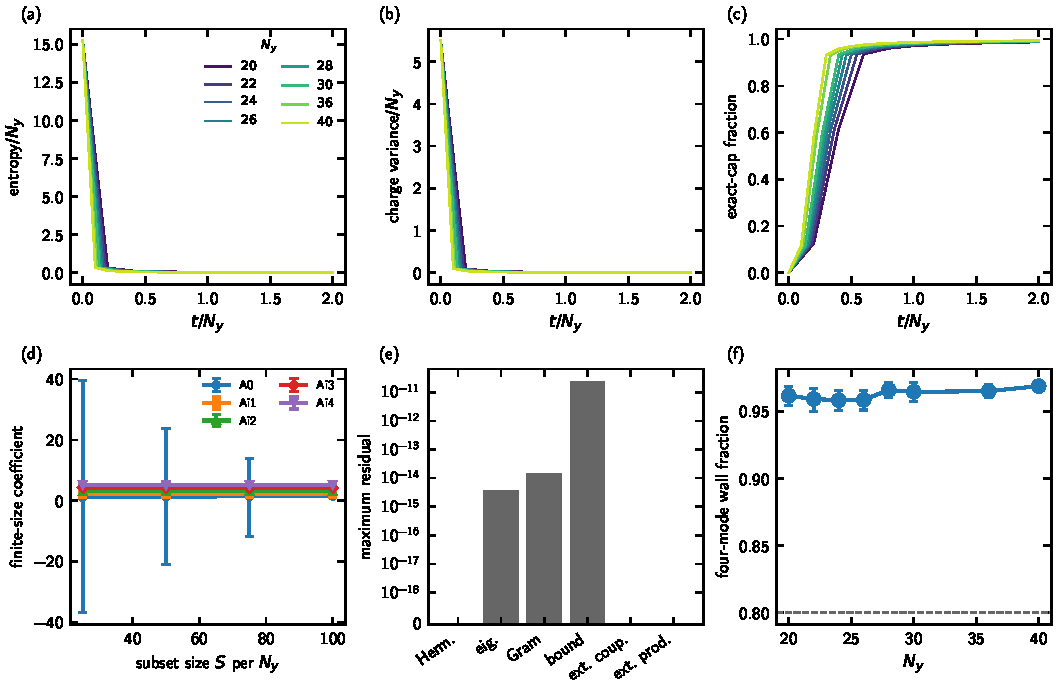
\includegraphics[width=\textwidth]{../../final_production_new_designs/04_maxmix_manybody_lyapunov_pilot/analysis_outputs/maxmix_manybody_lyapunov_nx20_ny20to40_s100_gpu_v2/many_body_lyapunov_v2_supplementary.pdf}
 \caption{Supplementary v2 diagnostics for the same $S=100$ independent Born trajectories and $T=2N_y$ campaign.  Panels show the trajectory-averaged active entropy, charge variance, exact-cap fraction, random without-replacement sample-size sensitivity of the finite-size coefficients, maximum numerical residuals, and aggregate four-mode wall fraction.  Curves use the saved estimator checkpoints; localization error bars are 95\% whole-trajectory bootstrap intervals with 2000 replicates.  The $S=100$ subset is the complete ensemble and therefore has no subset-selection interval.}
 \label{fig:v2-supplement}
\end{figure*}

\section{Interpretation and next experiment}

The v2 result separates three questions.  First, the Gaussian reconstruction is numerically and probabilistically consistent: occupations and record weights reproduce the saved many-body levels and the leading late-window rate.  Second, the low-cost sector is strongly localized at the two interfaces.  Third, the present depth is not long enough for a controlled Zabalo-style finite-size coefficient.  The latter failure is a convergence limitation, not evidence against the already established spatial boundary criticality.

The economical next experiment is a fresh $T=4N_y$, $S=100$ depth study at $N_y=20,30,40$.  It should repeat the same per-trajectory middle/late analysis at the longer depth before adding sizes or samples.  This note recommends that campaign but does not launch it.  The v2 outputs do not contain final covariance and random-number-generator state, so the extension cannot continue the existing trajectories and must rerun from $t=0$.

\section{Conclusion}

A maximally mixed Gaussian trajectory gives \(\hat V_{\boldsymbol m}\hat V_{\boldsymbol m}^{\dagger}/Z_{\boldsymbol m}\) directly.  In the completed v2 campaign, its occupations reconstruct the normalized many-body singular spectrum, and the cumulative Born log weight restores the common normalization.  All 800 trajectories pass provenance and numerical checks, same-window record closure is sub-percent, and the first four soft modes are 95--97\% wall-localized.  Nevertheless, every circumference fails at least one temporal-stability test, and the leading finite-size coefficient has the wrong sign and extreme sensitivity to fit range and subleading corrections.  The campaign validates reconstruction and boundary localization; it does not establish \(c_{\rm eff}\), absolute operator dimensions, or a stable anisotropy-free ratio.

\clearpage
\begin{thebibliography}{9}

\bibitem{Zabalo2022}
A.~Zabalo, M.~J.~Gullans, J.~H.~Wilson, R.~Vasseur,
A.~W.~W.~Ludwig, S.~Gopalakrishnan, D.~A.~Huse, and J.~H.~Pixley,
``Operator scaling dimensions and multifractality at measurement-induced transitions,''
arXiv:2107.03393v3 (2022).

\bibitem{Bhuiyan2026}
A.~Bhuiyan, H.~Pan, and C.-M.~Jian,
``Free-fermion dynamics with measurements: Topological classification and adaptive preparation of topological states,''
Phys. Rev. Research \textbf{8}, 023147 (2026).

\bibitem{CalabreseCardy2004}
P.~Calabrese and J.~Cardy,
``Entanglement entropy and quantum field theory,''
J. Stat. Mech. P06002 (2004).

\end{thebibliography}

\end{document}
